
\documentclass[a4paper,UKenglish,cleveref, autoref, thm-restate]{lipics-v2021}

\bibliographystyle{plainurl}% the mandatory bibstyle
\usepackage{booktabs}   %% For formal tables:
                        %% http://ctan.org/pkg/booktabs
\usepackage{subcaption} %% For complex figures with subfigures/subcaptions
                        %% http://ctan.org/pkg/subcaption

\usepackage{mathtools}
\usepackage{todonotes}
\usepackage{microtype}

\usepackage{complexity}
\usepackage{amsmath}
\usepackage{dsfont}

\usepackage{stmaryrd}
\usepackage{MnSymbol}
\usepackage{graphicx}




\newcommand{\problemx}[3]{
	\vspace{0.2cm}
\par\noindent\underline{\sc#1}\par\nobreak\vskip.2\baselineskip
\begingroup\clubpenalty10000\widowpenalty10000
\setbox0\hbox{\bf INPUT:\ }\setbox1\hbox{\bf QUESTION:\ }
\dimen0=\wd0\ifnum\wd1>\dimen0\dimen0=\wd1\fi
\vskip-\parskip\noindent
\hbox to\dimen0{\box0\hfil}\hangindent\dimen0\hangafter1\ignorespaces#2\par
\vskip-\parskip\noindent
\hbox to\dimen0{\box1\hfil}\hangindent\dimen0\hangafter1\ignorespaces#3\par
\endgroup
	\vspace{-0.2cm}
}

\newcounter{claimcounter}
\setcounter{claimcounter}{0}
\newtheorem{subclaim}{Subclaim}{}
\newtheorem*{theorem*}{Theorem}

\makeatletter

\usepackage{ textcomp } 

\usepackage{stmaryrd}
\usepackage{MnSymbol}
\usepackage{graphicx}

\usepackage{wrapfig}


\newcommand\sg[1]{\todo[inline,size=\scriptsize]{#1 - \textbf{Stefan}}}
\newcommand\mh[1]{\todo[inline,size=\scriptsize]{#1 - \textbf{Mathieu}}}
\newcommand\sgchanged[1]{{\color{red}{'1}}}
\newcommand\mhchanged[1]{{\color{blue}{'1}}}


\renewcommand{\A}{\mathcal{A}}
\newcommand{\B}{\mathcal{B}}
\renewcommand{\C}{\mathcal{C}}
\newcommand{\T}{\mathcal{T}}
\renewcommand{\G}{\mathcal{G}}
\renewcommand{\O}{\mathcal{O}}
\renewcommand{\R}{\mathbb{R}}
\newcommand{\Z}{\mathbb{Z}}
\newcommand{\N}{\mathbb{N}}
\newcommand{\Time}{\mathbb{T}}
\newcommand{\Const}{\mathsf{Consts}}
\newcommand{\PTA}{\textsc{PTA}}
\newcommand{\MSO}{\textsc{MSO}}


\renewcommand{\poly}{\mathrm{poly}}



\newcommand{\semi}[1]{\xRightarrow{'1}}




\title{Parity games in pushdown systems with pebbles} 

\titlerunning{Parity games in pushdown systems with pebbles} 

% \author{Stefan G\"oller}{University of Kassel \and School of Electrical Engineering and Computer Science \and Kassel, Germany }{stefan.goeller@uni-kassel.de}{}{The author was supported by the Agence Nationale de la Recherche grant no.  ANR-17-CE40-0010.}
\author{Mathieu Hilaire}{Université Paris-Saclay\and
CNRS\and
ENS Paris-Saclay\and
Laboratoire Méthodes Formelles (LMF)\and
Gif-sur-Yvette, France
}{hilaire@lsv.fr}{}{This work was partly done while the author was supported by the 
Agence Nationale de la Recherche grant no.  ANR-17-CE40-0010.}

\authorrunning{M. Hilaire} 

\Copyright{M. Hilaire} 

%\ccsdesc[500]{Theory of computation~Timed and hybrid models}
%\ccsdesc{Theory of computation~Automata over infinite objects}
\ccsdesc[500]{Theory of computation~Automata extensions}

\keywords{Parity Games, Computational Complexity, Pushdown systems, Pebble Alternating Two Way Automata}



\category{} 

\relatedversion{}
% \relatedversiondetails{Full Version}{}

\acknowledgements{The author would like to thank Benedikt Bollig and Stefan G\"oller for helpful discussions and feedback.}


\ArticleNo{70}
\begin{document}

\maketitle


\begin{abstract}
	We investigate the decidability and complexity of
	parity games over an extension of pushdown systems.
	More specifically, we consider pebble pushdown systems, in
	which pebbles can be used to remember some stack content already visited,
	and compared against.
	We determine decidability of the problem, and provide a nonelementary lower bound. 
\end{abstract}

\section{Introduction}

\subsubsection*{Background}



Stack-based automata are a popular formalism for modeling the sequential behavior of computer programs. 
Pushdown systems are probably the most studied models of stack-based automata.
They are
finite automata 
 extended with a stack that can be manipulated by pushing or popping stack symbols from some finite set, and can use the top of the stack to decide which transition to take next.
\textcolor{black}{To underline the fact that we are concerned with the graph of configurations and not the language recognized, we use the name pushdown system rather than pushdown automaton.}
Pushdown systems can be used to model the behavior of recursive programs and,
as a result, a variety of 
 program analysis questions can be reduced to decision problems for games on pushdown systems.
They have applications for instance in inter-procedural control-flow analysis of recursive programs \cite{esparza1999automata, reps2005weighted}.





Two player games can be used in particular to
 represent the
interaction of a program with some environment, with the first player representing the program while the second player represents the environment. A winning condition then expresses a property required to hold however the environment behaves. Finding a winning strategy for the first player
thus provides some way 
 to ensure that the desired 
property, as expressed by the winning condition,
always holds \cite{arnold2003games}.


Games on the graphs of pushdown systems have been extensively studied.
It is known in particular from \cite{walukiewicz1996pushdown} that deciding the winner of a parity game on a graph of a pushdown system is an ${\sf EXPTIME}$-complete problem.
Several generalizations of the pushdown systems 
have been studied in depths, including
tree-pushdown systems \cite{guessarian1983pushdown}, ordered
multi-pushdown systems \cite{breveglieri1996multi, atig2012model}, annotated higher-order pushdown systems \cite{maslov1976multilevel, broadbent2012saturation}, and
strongly normed multi-pushdown systems \cite{czerwinski2012reachability}.




We consider here a different approach to extending pushdown systems, by allowing them to test the stack content against precise values.
Pushdown systems which can test the stack content against regular-expressions are
equivalent to pushdown systems,
so pushdown systems which can test the stack content against specific words are too.
We consider instead checks against unspecified word values that can be instantiated one after the other,
providing the pushdown systems the ability to
store information on some stack contents for later comparisons.



Hence we propose in this paper to extend pushdown systems with a set of pebbles.
Compared to pebble word automata, instead of using pebbles
as markings on their input, pebble pushdown systems have the ability to lift or drop pebbles
on their universe of stack contents. Dropping a pebble records the current stack content with an available pebble until it is lifted. Lifting a pebble then makes it available again.


A pebble automaton is a two-way finite state automaton that uses a fixed, finite number of
pebbles that it can drop on, and lift from 
words, using them as markers.
Pebble automata recognize regular languages only, provided the life times of the pebbles, i.e. the times between dropping a pebble and lifting it again, are properly nested
\cite{globerman1996complexity, engelfriet1999tree}.
Automata with nested pebbles were also introduced
for tree-walking automata. 
It is known that tree-walking automata do not recognize all regular tree languages \cite{bojanczyk2008tree}, the main trouble being that the tree-walking automata get lost rather easily.
Using pebbles is a remedy against getting lost along a tree, but 
the unrestricted use of pebbles leads to a class of tree languages much larger than the
regular tree languages, in fact to all tree languages in $\NSPACE(log ~ n)$.
Thus, in both pebble word automata and pebble tree-walking automata, the placement of the pebble follows a strict stack discipline, and our model will follow this strict stack discipline too.



One motivation to the study of pebble pushdown systems is their ability to compare a stack content against some later stack content.
Similar type of storage for later comparison has already been used for instance
in register pushdown systems. Introduced in \cite{murawski2017reachability}
 as an extension of pushdown systems that 
 can keep data values in
 a set of registers and a stack,
register pushdown systems
enable
manipulation of
data values from an infinite domain,
and have applications for instance for
malware detection and XML schema
checking \cite{senda2021forward, senda2021ltl}.





Another closely related formalism is that of alternating tree automata with nested pebbles, as we 
consider in more details in Section 4. The approach of extending tree automata with pebbles was used in \cite{milo2000typechecking} to show that the XML typechecking problem is decidable, and in \cite{karhumaki2012jewels} to recognize first-order logic on trees. In both cases however, the input trees considered are finite, while 
simulation of plays in pebble pushdown graphs
requires the use of pebble alternating tree automata working on infinite trees
since the stack of a pebble pushdown system is in general unbounded.






The aim of the present paper is to study the decidability and complexity of
deciding
the winner of a parity game on a graph of a pushdown system with  
pebbles.




\subsubsection*{Contributions}


Our main result states that
deciding
the winner of a parity game on a graph of a pebble pushdown system
is decidable but nonelementary.
The contribution is two-fold. 




	For the nonelementary lower bound,
we reduce the $\FO$ satisfiability problem on words, known to be nonelementary
from \cite{Sto74}, to the
problem of deciding whether a player has a winning strategy. 

	For the main contribution, we use pebble alternating two-way tree automata to solve pebble pushdown parity games.
Alternating two-way tree automata with parity winning conditions have been used in the past to solve parity games on pushdown graphs \cite{cachat2002two}. We show that pebble alternating two-way tree automata can similarily be used to solve parity games on pebble pushdown graphs.
We then prove  decidability 
by 
a reduction
 to the problem of model-checking $\MSO$ on a well chosen structure, whose decidability is
 guaranteed by
Muchnik's Theorem~\cite{Wal96}.



\subsubsection*{Overview}

In Section 2, we provide general notations and preliminary definitions. Section 3 will deal with the introduction of pebble pushdown games.
Section 4 is devoted to using pebble alternating tree automata with parity acceptance condition to solve pebble pushdown system parity games. We leave the proof of decidability itself  for Section 5.
Section 6 at last shows a nonelementary lower bound for the problem.




\section{Definitions}


\newcommand{\LCM}{\mathsf{LCM}}
\newcommand{\LOGSPACE}{\mathsf{LOGSPACE}}
\renewcommand{\MSO}{\mathsf{MSO}}
\newcommand{\SO}{\mathsf{SO}}

By $\Z $ we denote the {\em integers} and by $\N=\{0,1,\ldots\}$ we denote the {\em naturals}.
% For every $a,b\in\Z$ with $a\leq b$ we define $[a,b]=\{k\in\Z\mid a\leq k\leq b\}$.
% For every $n\geq 1$ we define $n\Z=\{n\cdot z\mid z\in\Z\}$.
% For every number $n\in\N$ we define $\log(n)=\min\{i+1\mid i\in\N, n\leq 2^i\}$, which is the smallest number of bits necessary to write down $n$ in binary.
For every finite alphabet $A$, $A^*$ is the set of finite
words with letters in  $A$, $A^\omega$ is the set of infinite words with letters in $A$, and
%by
 $A^\infty = A^\omega \cup A^*$. We denote the empty word in $A^*$ by $\epsilon$.
%For all $a\in A$ and all $w\in A^*$ let $|w|_a$ denote the number of occurrences of the letter $a$ in $w$.
%
% For every finite set $M\subset\N\setminus\{0\}$ let $\LCM(M)=\min\{n\geq 1\mid \forall m\in M\setminus\{0\}: m|n\}$ denote the least common multiple of the elements in $M$. 
% For any $j \in \N$ let $\LCM(j)=\LCM([1,j])$ denote the least common multiple of the numbers $\{1,\ldots,j\}$.

 For any two sets $X$ and $S$, let $X^S$ denote the set of all functions from $S$ to $X$.
For any set $S$ let 
%$\mathscr{P}(S) = \{ X \mid X \subseteq S \}$
$\mathcal{P}(S) = \{ X \mid X \subseteq S \}$
denote the power set of $S$.
%
A {\em partial function} $f$ from a set $X$ to a set $Y$ is a function defined on a subset $C$ of $X$ (possibly $X$ itself) with output values in $Y$. We extend the domain of a partial function to the whole set
by considering it as returning the bottom element $\bot$ when it is undefined.




A {\em graph} $G=(V,E)$ is a finite set of graph vertices $V$ with a set of graph edges $E \subseteq V \times V$. 
% Two graphs $G = (V,E)$ and $G'=(V',E')$ with sets of graph vertices $V=V'=V_n=\{1,2,...,n\}$ are said to be {\em isomorphic} if there is a permutation $\rho$ of $V_n$ such that $(u,v)$ is in the set of graph edges $E$ iff $(\rho(u),\rho(v))$ is in the set of graph edges $E'$.
%%%
%
For any set $V$, and a given infinite sequence $\pi = v_0 v_1 \ldots \in V^\omega$ of elements of $V$, we define the set 
$\text{\textit{Inf}}(\pi)$ of elements occurring infinitely often in $\pi$ as
$\text{\textit{Inf}}(\pi) = \{ v \in V \mid \forall i, \exists j > i, ~ v_j = v \}$. 






\subsection{Logics}

We now briefly review some standard definitions from mathematical logic.

\begin{samepage}
\begin{definition}
 A {\em vocabulary} $\tau$ is a set of relational symbols (denoted $P_1, P_2, \ldots $), each of which has a specified
 arity. A symbol $P \in \tau$ is called monadic if its arity is one, i.e., if it is used to
 denote sets.
%
A {\em $\tau$-structure} %(also called a {\em model})
%
$$ \mathfrak{A} = (A,	( P^{\mathfrak{A}} )_{P \in \tau})$$
%
consists of a set $A$ together with an interpretation of
 each $k$-ary relational symbol $P$ from $\tau$ as a $k$-ary relation on $A$; that is, a
set $P^{\mathfrak{A}} \subseteq A^k$.
% A structure $\mathfrak{A}$ is called finite if $A$ and $\sigma$ are finite sets. 
% The {\em universe} of a structure is typically denoted by a Roman letter corresponding to the name of the structure; that is, the universe of $\mathfrak{A}$ is the set $A$, the universe of $\mathfrak{B}$ is $B$, and so on. We shall also occasionally write $a \in \mathfrak{A}$ instead of $a \in A$.\newline
%
\end{definition}
\end{samepage}


%\noindent As an illustration, if $\tau$ consists of a single relational symbol $E$ of arity $2$, graphs are possible $\tau$-structures. 




% Next, we define the  monadic second-order logic, or $\MSO$.

Next, we define monadic second-order formulas over a vocabulary $\tau$, or $\MSO[\tau]$ for short. %We define free variables, and the semantics of $\MSO(\tau)$ formulas.

\begin{samepage}
\begin{definition}\label{MSO}
We assume countably infinite sets of first-order variables {\em Var}
and of second-order variables {\em VAR}. First-order variables
will be typically denoted by $x, y, z, \ldots,$ with subscripts and superscripts,
whereas second-order variables will be typically denoted by $X, Y, Z, \ldots ,$
using subscripts and superscripts as well. We
inductively define %terms and 
formulas of the monadic second-order logic
over vocabulary $\tau$ %as follows: 
by the grammar:
$$ \phi :=  P(x_1 , \ldots , x_k) \mid x_1 = x_2 \mid X(x) 
		\mid \phi \vee \phi \mid \phi \wedge \phi \mid \neg \phi 
		\mid \exists x ~ \phi \mid  \forall x ~ \phi
		\mid \exists X ~ \phi \mid  \forall X ~ \phi		$$
where $P \in \tau$ is a $k$-ary relational symbol, $X \in \text{VAR}$, and $x, x_1, \ldots, x_k \in \text{Var}$.
\end{definition}
\end{samepage}

A formula that does not use existential ($\exists$) nor universal ($\forall$) quantifiers
is called {\em quantifier-free}.
%
% Given a set of formulas $S$, formulas constructed from formulas in $S$ using only the Boolean connectives $\vee$, $\wedge$, and $\neg$ are called {\em Boolean combinations} of formulas in $S$.
%
We shall use the standard shorthand $\phi  \to \psi $ for $ \neg \phi \vee \psi $ 
and $\phi \leftrightarrow \psi $ for
$(\phi  \to \psi ) \wedge (\psi  \to \phi )$. 


If $\overrightarrow{x}$ is the tuple of all the free first-order variables of $\phi$,
and $\overrightarrow{X}$ is the tuple of all the free second-order variables of $\phi$ 
we write $\phi(\overrightarrow{x},\overrightarrow{X})$. A {\em sentence}
is a formula without free variables. We use the standard semantic of $\MSO$,
see Appendix~\ref{MSO appendix} for a more thorough induction over the formula.\\





Concerning the logic $\MSO$, we are interested in the following decision problem.

\problemx{$\MSO[\tau]$ model-checking}
{A $\tau$-structure $\mathfrak{A}$ and a $\MSO[\tau]$-sentence $\phi$.}
{Does $\mathfrak{A} \models \phi $ ?\newline}


\textcolor{black}{We define the problem in a general abstract manner, instead of focusing on particular representation for the input, since we will consider many structures of infinite size.}



{\em First-order logic over a vocabulary $\tau$} ($\FO[\tau]$ for short) is the fragment of $\MSO$ which is restricted to first-order quantifiers and variables: quantification is permitted only over individuals, and no second-order variables are used. 







\subsection{Parity Games}

We first recall the definition of  two  player parity  games.
Two players, player $0$ and player $1$, move along an arena $\mathcal{G}=(V_0,V_1,E,\Omega)$ which is a labelled graph, composed of
two  disjoint  sets of vertices, $V_0$ and $V_1$ respectively associated with player $0$ and player $1$, 
a set of edges $E \subseteq V \times V$, where $V=V_0 \uplus V_1$,
% We require that the out-degree of each vertex is at least one. This ensures that every finite path in (V, E) can be prolonged.
and a mapping $\Omega:V \to \{0,1, \ldots, m\}$,
$m < \omega$, which
assigns a priority to each vertex. %Then the {\em initialized game} $(\mathcal{G}, v_I)$ is given with an initial vertex $v_I \in V$.



A {\em partial play} of $\mathcal{G}$ is a sequence of vertices $v_0 v_1 \ldots \in V^\infty$ connected by the transition relation, i.e. such that $(v_i, v_{i+1}) \in E$.


A {\em play} of $\mathcal{G}$ is a partial play that is {\em maximal} in the following sense: if it is finite, then the last vertex $v_k$ is such that for all $v' \in V$, $(v_k, v') \notin E$. Else, the play is an infinite sequence $ \pi  = v_0 v_1 \ldots \in  V^{\omega} $.


We consider min-parity games: in order to find out who wins a play, we need to take a
look at the positions which are reached infinitely often and compute their priorities using 
$\Omega$.
Player $0$ wins the play $\pi$  iff  $\min( \{ \Omega(v) \mid v \in \text{\textit{Inf}}( \pi) \})$ is even, else, player $1$ wins. The winner of a finite play is the player whose opponent is unable to move, i.e. the winner of a play such that the last vertex of the play is in $V_{0}$ (resp. $V_1$) is player $1$ (resp. player $0$). 



A {\em strategy} $\sigma_i : V^* V_i \to V$ for player $i \in \{ 0,1\}$ is a function that, given a sequence of vertices $ w v$  with $w\in V^*$ and $v \in V_i$,
provides, if possible, a successor $v'$ such that $(v,v') \in E$.
A strategy is called {\em memoryless} if its output only depends on the final vertex of the sequence $v \in V_i$, i.e. if there exists a function $f_i : V_i \to V$ such
that for all $w\in V^*$, $v \in V_i$, we have $\sigma_i(wv) = f_i(v)$.

A partial play $\pi$ is {\em consistent} with a strategy $\sigma_i$ if sequences of vertices that end in $V_i$ along this play all have successors according to the strategy. Given a starting vertex $v_I$,   a strategy $\sigma_0$ for player $0$ and a strategy $\sigma_1$ for player $1$, the play
starting with $v_I$ that is consistent with both strategies is unique and is called the {\em resulting play} of $\sigma_0$ and $\sigma_1$ starting from $v_I$. It is 
denoted by $\pi(v_I, \sigma_0, \sigma_1)$.


A strategy $\sigma_i$ for player $i$ from position $v_I \in V$ is a {\em winning strategy from $v_I$} if 
no matter which
strategy $\sigma_{1-i}$ the other player pursues,
% the resulting play  starting from $v_I$  
%  results in 
% player $i$ winning.
player $i$ wins the play $\pi(v_I, \sigma_0, \sigma_1)$.


The above definitions are essentially the same for finite and infinite arenas.
%
%
In this paper we are going to concern ourselves with parity games over potentially infinitely large arenas, \textcolor{black}{thus we define the following decision problem in a general abstract manner. In particular, we do not discuss representation of the input}. 

\begin{samepage}
\problemx{Solving parity game}
{An arena $\mathcal{G}=(V_0,V_1,E,\Omega)$, an initial vertex $v_I \in V$.}
{Does player $0$ have a winning strategy from $v_I$ in the parity game $\mathcal{G}$?\newline}
\end{samepage}

One important property of parity games is that of {\em memoryless determinacy}: for a parity game and an initial vertex $v_I \in V$, one of the players has a memoryless winning strategy from $v_I$ \cite{zielonka1998infinite}.




\section{Pebble pushdown games}

In this section, we extend pushdown systems with a set of pebbles. 
Pebble pushdown systems will have the ability to lift or drop pebbles on their universe of stack contents according to a strict stack discipline. A \textit{drop} simply records the current stack content with a fresh pebble (such a pebble should be available) and a \textit{lift} pops the last dropped pebble. One can think of a pebble as a register that can store a stack content.




\begin{definition}
An $n$-pebble pushdown system ($n$-PPDS) is a tuple $\mathcal{Z} = (Q, \Gamma,  \Delta )$
where:
\begin{itemize}
\item $Q$ is a {\em finite set of control states},
\item $\Gamma$ is a {\em finite stack alphabet},
% \item $\$ \notin W$ is an {\em initial stack symbol},
\item  $\Delta   \subseteq  Q  \times (\Gamma \biguplus \{ \$ \})  \times \{ 0, 1, \ldots, n\} \times \mathcal{P}(\{ 1, \ldots, n\}) \times Q  \times (\Gamma^* \cup \{ \! \! \text{\textit{lift}}, \text{\textit{drop}}\})$ is a {\em finite transition relation}, where ${\$ \notin \Gamma}$ is some bottom of stack symbol.
\end{itemize}
\end{definition}


A transition in an $n$-pebble pushdown system works like a transition in a pushdown system that additionally manages the $n$ pebbles.
The idea of a transtion $(q, a, i, S, q', \theta) \in \Delta$
is that, if the automaton $\mathcal{Z}$ is in state $q$ with pebbles $1,\ldots, i$ dropped \---- or without pebble dropped if $i = 0$ \---- with top stack symbol $a$, and stack content which corresponds to the stack contents of the pebbles from $S$ and only these pebbles, then
$\mathcal{Z}$ goes to state 
$q'$ and makes modifications to the stack or the pebbles according to
$\theta$.



A {\em pebble set} of $\mathcal{Z}$ is a set $P \subseteq \{ 1, \ldots, n\}$. For a stack alphabet $\Gamma$, a 
{\em $P$-pebble assignment} is a function which maps each $j \in P$ to a word in $\$\Gamma^*$.
For $0 \leq i \leq n$, an {\em $i$-configuration} is a tuple $(q, w, f )$, where 
$q$ is a state,
$w \in \$\Gamma^*$, and
$f$ a $\{ 1, \ldots , i \}$-pebble assignment \---- $f$ is the $\emptyset$-pebble assignment in case $i=0$. 
We call  $q$ the current state, $w$ the current stack, and
$f$ the current pebble assignment. 
We also write $(q,w, w_{1} , \ldots , w_{i} )$ if 
$f(j) = w_j$, for each
$j \leq i$.


The set of configurations is the union of all $i$-configurations for $0 \leq i \leq n$. The transition graph of $\mathcal{Z}$ is $(V,E)$, where $V$ is the set of configurations. %and $E$ is such that
Moreover, 
for all $(q, a, i, S, q', \theta) \in \Delta$, with $a \in \Gamma$ (respectively $ \! a = \$ $),
 for all words $w \in \$ \Gamma^*$, and for all $\{ 1, \ldots , i \}$-pebble assignments 
 
 \begin{samepage}
\noindent
 $f$ such that $f(j) = wa$ (respectively $f(j)= \$ $) for each
$j \in S$ 	and
 $f(j) \neq wa$ (resp. $f(j) \neq \$ $) for each $j \in \{ 1, \ldots , i \} \setminus S$,
%the following holds
we include in $E$ the following transitions:
\begin{itemize}
\item if $\theta \in \Gamma^*$, 
$((q,wa,f), (q',w\theta, f)) \in E $ \\
(respectively, $((q,\$,f), (q',\$\theta, f)) \in E $),
\item if $ \theta = \text{\textit{drop}}$, 
$((q,wa,f), (q',wa, f')) \in E $  \\
(respectively, $((q,\$,f), (q',\$, f')) \in E $),\\
where $f'$ is the $\{ 1, \ldots , i, i+1 \}$-pebble assignment such that
$f'(j) = f(j)$ for each
$j \leq i$, and $f'(i+1) = wa$ (respectively, $f'(i+1) = \$$), and
\item if $\theta = \text{\textit{lift}}$, and $ i \in S $%$i>0$
, 
$((q,wa,f), (q',wa, f')) \in E $ \\ 
(respectively, $((q,\$,f), (q',\$, f')) \in E $),\\
where $f'$ is the $\{ 1, \ldots , i - 1 \}$-pebble assignment such that
$f'(j) = f(j)$ for each
$j < i$.
\end{itemize}
\end{samepage}


This defines a graph  $(V,E) $. 
%
To obtain
a parity game, it remains to define the sets $V_0$ and $V_1$ associating the vertices
to the two players, and the priorities of the configurations. One fixes a disjoint
union
 $Q = Q_0  \biguplus Q_1 $. Then 
 $V_0$ is the set of configurations with current state in $Q_0$ and 
 $V_1$ is the set of configurations with current state in $Q_1$.
The mapping  $\Omega$ is first
defined on $Q$, then  $\Omega (q,w,f) =  \Omega (q)$,  for all words $ w  \in \$ \Gamma^*$, all pebble assignments $f$, and 
$q  \in  Q$. So the player and the
priority only depend on the control states of $\mathcal{Z}$. 
This defines the {\em $n$-pebble pushdown game} $ \mathcal{G}_{\mathcal{Z}, Q_0,Q_1,\Omega}$.
The starting configuration is defined if we also fix an initial state 
$q_I  \in  Q$ as $v_I = (q_I, \$, f_I)$, where $f_I$ is the $\emptyset$-pebble assignment. \newline



The main problem we are interested in in this article is the following decision problem.

\problemx{Solving pebble pushdown parity game}
{A pebble pushdown system $\mathcal{Z}= (Q,\Gamma, \Delta )$, a disjoint
union $Q = Q_0  \biguplus Q_1 $, a priority mapping $\Omega$, an initial state $q_I \in Q$% and initial stack symbol $w_I \in W$
.}
{Does player $0$ have a winning strategy from $(q_I,\$, f_I)$ in the  parity game
$ \mathcal{G}_{\mathcal{Z}, Q_0,Q_1,\Omega}$ ?}
%$(\mathcal{G}_{\mathcal{Z}}, \Omega)$ ?\newline}









\section{Tree Automata}

In this section, we use pebble alternating two-way tree automata to solve pebble pushdown parity games. 
We introduce first alternating two-way tree automata, then pebble alternating two-way tree automata,
then explain the reduction. Decidability questions concerning pebble alternating two-way tree automata
are dealt with in Section~\ref{section decidability}.



\subsection{Alternating two-way tree automata}

Given a finite set $\Gamma$ of directions, a $\Gamma$-tree is a prefix closed set 
$T  \subseteq \Gamma^*$,
i.e., if $x.d  \in  T$, where 
$x  \in  \Gamma^*$ and $d  \in  \Gamma $, then $x  \in  T $. 
We will sometimes forget the “.” of the concatenation. 
The elements of $T$ are called {\em nodes}, the
 empty word  $\epsilon$
% word $\$ $
  is the {\em root} of $T $. For every $x.d  \in  T$, $d  \in  \Gamma$ the node $x$ is the
unique {\em parent} of $x.d$, and $x.d$ is a {\em $d$-child} of $x$. The {\em direction} of a node $x.d$
$( \neq   \epsilon )$ 
%$(\neq \$ )$
is $d$. 
The full infinite tree is 
$T = \Gamma^*$. A {\em path (branch)} of a tree $T$ is
a sequence  $\beta   \in  T^{\infty}$  such that 
$ \beta  = u_0 u_1 \ldots u_n$ or 
$ \beta  = u_0 u_1 u_2 \ldots$, where
$u_0 =  \epsilon$  and
 $\forall i < n,  \exists d  \in  \Gamma$, $u_{i+1} = u_i.d$. 
 A path can be finite or infinite.



For a finite set $X$, $\mathcal{B}^+ (X)$ is the set of positive Boolean formulas
over $X$ (i.e., Boolean formulas built from elements in $X$ using only $\wedge$ and $\vee$),
where we also allow the formulas $\text{\textit{true}}$ and $\text{\textit{false}}$. For a set $Y  \subseteq  X$ and a
formula $ \vartheta   \in  \mathcal{B}^+ (X)$, we say that $Y$ satisfies $ \vartheta$  iff assigning $\text{\textit{true}}$ to elements in
$Y$ and $\text{\textit{false}}$ to elements in $X \setminus Y$ makes  $\vartheta $ true.

The set $\text{\textit{types}}(\Gamma) = \{r \} \cup \Gamma$ 
describes the possible types of a node in the full infinite tree $\Gamma^*$. 
Here $r$ stands for the root, $\gamma \in \Gamma$ for a $\gamma$-child.

To navigate through the tree let $ext(\Gamma ) := \Gamma \biguplus \{ \epsilon , \uparrow \}$ be the extended set of directions: The symbol $\uparrow$ means “go to parent node”, 
and  $\epsilon$  means “stay on the present
node”. Formally we define $ \forall u  \in \$ \Gamma^* , d  \in  \Gamma, u.\epsilon  = u$ and $u.d. \! \uparrow= u$, while the node 
$ \epsilon . \! \uparrow $ is not defined.




\begin{definition}
An alternating two-way automaton over
 $\Gamma$-trees (ATWA) is a tuple
$\mathcal{A} = (Q,  \delta , q_I , 
\Omega)$ where
\begin{itemize}
\item $Q$ is a {\em finite set of states},
\item $\delta  : Q  \times  
%
\text{\textit{types}}(\Gamma)
%W \cup \$
  \to  \mathcal{B}^+ (Q \times ext(\Gamma))$ is a {\em transition function},
\item $q_I$ is an {\em initial control state}, and
\item $\Omega: Q \to \{ 0, 1, \ldots, m\}$ is a {\em priority function}.
\end{itemize}
\end{definition}



The idea of a transition $ \delta (q, a) = ( q',\uparrow ) \wedge (q'',d)$ with $a,d\in\Gamma$ is the following: 
if the automaton
$\mathcal{A}$ is in state $q$ on the node $x.a$ of the 
tree $T$, it will send a “copy” of $\mathcal{A}$  in state $q'$ to the node $x$ and
another “copy” in state $q''$ to $x.a.d$. 
After that the two copies are
running independently. They may come again to the same node with two different
states.


More precisely a run of an alternating two-way automaton $\mathcal{A}$ over a tree
is
a tree $T_r$ in which every node is labelled by an
element of $Q \times \Gamma^*$. The latter tree is like the unfolding of the run, its structure
is different from the tree $\Gamma^*$, and its set of directions range rather on the naturals smaller than $|Q|*|ext(\Gamma)|$; a node in $T_r$ labelled by $(q,x)$ describes a “copy”
of the automaton that is in state $q$ and is situated at the node $x$ of $\Gamma^*$. 
Note
that many nodes of $T_r$ can correspond to the same node of $\Gamma^*$, because the
automaton can come back to a previously visited node. 
The label of a node
and its successors have to satisfy the transition function,
that is, for a node $y$ of $T_r$ labelled by $(q,x)$, and $\delta(q,t)= \vartheta$ where $t$ is the type of $x$, there is a (possibly empty) set 
 $Y = \{ (q_0,d_0),(q_1,d_1), \ldots (q_\ell, d_\ell) \}  \subseteq  Q \times ext(\Gamma)$, such that $Y$ satisfies  $\vartheta $, and for all
$(q_i,d_i)  \in  Y$, the node $y$ has a corresponding son $y.i$ labelled by $(q_i,x.d_i)$. Finally, the root of $T_r$ is labelled by $(q_I,\epsilon)$.



Remember that $x.d$ can be $x. \epsilon$  or $x. \! \uparrow$, and the latter is defined only if 
%$x \neq \$ $.
$x  \neq   \epsilon $.
So the run cannot go up from the root of the input tree. Note that it cannot use a
transition  $\delta (q, a) = \text{\textit{false}}$ since the formula $\text{\textit{false}}$ cannot be satisfied.
A run $T_r$ is accepting if all its infinite paths satisfy the parity acceptance 
condition
given by the priority function. 
% The finite paths of a run that end with a transition $ \vartheta $ equivalent to  $true$, which is viewed as successful termination. 
An infinite path $ \beta   \in  T_r^{\omega}$  satisfies the acceptance condition iff the smallest priority appearing infinitely often in
%this path
the sequence $\gamma$ of corresponding labels
 is even, i.e.
%$\min ~ \text{\textit{Inf}}( \Omega (r( \beta ))) $
 $\min(\{ \Omega(q) \mid (q,x) \in \text{\textit{Inf}}(\gamma) \} $ is even. 
Such
a path in the run consists of following only one “copy” of the automaton. 


% The generalization of twa with nested pebbles came recently, by two independent motivations: On the one hand, with the advancement of XML theory, finite state recognizers (with name n-pebble tree automata) were used in [21] to show that the XML typechecking problem is decidable. On the other hand, the concept of n-pebble tree-walking automata (n-ptwa) were defined in [9] to recognize first-orderlogic on trees.  Later, in [10]n-ptwa were extended with a more general pebble handling.


\subsection{Alternating two-way tree automata with pebbles}

Informally an $n$-pebble alternating two-way tree automaton works much like an alternating two-way tree automaton, but extended with a fixed set of pebbles, numbered from $1$ to $n$ that it can place on the tree. 
% At each time, pebbles $1,\ldots, i$ are placed on some nodes of the tree, for some $i \in \{1, 2, \ldots , n \}$, or no pebble are placed on the tree. 
To navigate through the tree the automaton can stay at the current node, move to its parent, to its 
 children, it can lift a pebble or place a pebble on the current node.
 Which of these transitions can be applied depends on the current state, the set
 of pebbles at the current node, 
and the type of the current node (root, $\gamma$-child for $\gamma \in \Gamma$). 
Operations $\text{\textit{lift}}$ and $\text{\textit{drop}}$ manage the
pebbles much like in pebble pushdown systems.
We indicate the possible kinds of moves of a pebble automaton by elements of the set 
$ext_2(\Gamma) = ext(\Gamma) \biguplus \{ \text{\textit{lift}}, \text{\textit{drop}}\}$.
% Clearly $\text{\textit{drop}}$ refers to dropping a pebble and $\text{\textit{lift}}$ to lifting a pebble. Note that the notation is  unambiguous by virtue of the stack discipline. 
% Finally recall that if $S$ is a set then $\mathcal{P}(S)$ denotes the powerset of $S$.

\begin{samepage}
\begin{definition}
For $n\geq 0$, an $n$-pebble alternating two-way automaton ($n$-PATWA) over  
$\Gamma$-trees is a tuple
$\mathcal{A} = (Q,   
\delta , q_I , 
\Omega)$ where
\begin{itemize}
\item $Q$ is a {\em finite set of states},
\item $\delta  : Q  \times \{ 0, 1, \ldots, n\} \times \mathcal{P}(\{ 1, \ldots, n\}) \times 
\text{\textit{types}}(\Gamma)
  \to  \mathcal{B}^+ (Q \times ext_2(\Gamma))$ is a {\em transition function},
\item $q_I$ is an {\em initial control state}, and
\item $\Omega : Q \to \{ 0, 1, \ldots, m\}$ is a {\em priority function}.
\end{itemize}
\end{definition}
\end{samepage}
 
 
The idea of a transition in a $n$-pebble alternating two-way tree automaton works like a transition in an alternating two-way tree automaton,
except the transition has additional conditions on the pebble assignment, and additional moves for taking care of the pebble.
Consider for instance 
that the automaton
 $\mathcal{A}$ is on the node $x.a$, in state $q$, pebbles $1, 2$ are on the tree, and exactly pebble $1$ is placed on the node $x.a$.
Then a transition
$\delta(q, 2, \{ 1\}, a) =  (q',\uparrow) \wedge (q'',\text{\textit{drop}})$
 will send a “copy” of $\mathcal{A}$  in state $q'$ to the node $x$ and
another “copy” in state $q''$ to $x.a$ with both pebble $1$ and pebble $3$ placed on the node. 
After that the two copies are
running independently.






%A {\em pebble set} of $\mathcal{A}$ is a set $P \subseteq \{ 1, \ldots, n\}$. 
For a tree structure $T$, a 
{\em $P$-pebble assignment} for a pebble set $P$ is a function which maps each $j \in P$ to a node in $T$.
For $0 \leq i \leq n$, an {\em $i$-configuration} is a tuple $(q, x, f )$, where $x$ is a node, $q$ a state and
$f$ a $\{ 1, \ldots , i \}$-pebble assignment \---- $f$ is the $\emptyset$-pebble assignment in case $i=0$. 
We call $q$ the current state, $x$ the current node, and
$f$ the current pebble assignment. 
We also write $(q, x, x_{1} , \ldots , x_{i} )$ if 
$f(j) = x_j$, for each
$j \leq i$.






Then, formally, a run of an $n$-pebble alternating two-way automaton $\mathcal{A}$
over a tree is a tree $T_r$ in which every node is labelled by 
an $i$-configuration,
for some $i \in \{0, 1, \ldots, n\}$. A node in $T_r$ labelled by $(q, x, x_{1}, x_{2}, \ldots, x_{i})$ describes a “copy” of the automaton that is in state $q$, and is situated on the node $x$ of $\Gamma^*$, with the pebbles up to $i$ already dropped, with the $j$-th pebble for $j \leq i$ dropped on the node $x_{j}$.

The label of a
node and its successors have to satisfy the transition function. % However, recall there are restrictions on the drop-operation and the lift-operation : only
% the pebble with the number $i$ can be lifted and only the pebble with number $i - 1$ can be
% placed.
Formally, this works much the same way as for alternating two-way tree automata; 
that is, the root of $T_r$ is
labelled by $(q_I,\epsilon, f_I )$, and, for a node $y$ of $T_r$ labelled by an $i$-configuration $(q, x, f)$, and 
for
$\delta(q, i, S, t) = \vartheta$ where $t$ is
the type of $x$, 
and $f(j) = x$ for each $j \in S$, and $f(j) \neq x$ for each $j \in \{1,\ldots,i \} \setminus S$,
there is a (possibly empty) set 
$Y \subseteq Q \times ext_2(\Gamma )$, such that $Y$ satisfies $\vartheta$,
and for all $(q',d) \in Y$, the node $y$ has a corresponding son
labelled with %$(x.d, q', f')$, where
\begin{itemize}
\item if $d \in ext(\Gamma)$,
the $i$-configuration $(q ', x.d , f)$,
%
\item if $d = \text{\textit{drop}}$, the $(i+1)$-configuration  $ (q', x, f')$, where the domain of $f'$ is $\{ 1, \ldots, i, i+1\}$, $f'$ is equal to $f$ on the domain of $f$, and $f'(i+1) =x$, and
%
\item if $d = \text{\textit{lift}}$
and $f(i) = x$, i.e. if the pebble $i$ is on the current node%
, the $(i-1)$-configuration $(q', x, f')$, where $f'$ is the restriction of $f$ to $\{1, \ldots, i-1 \}$.
\end{itemize}








A run $T_r$ is {\em accepting} if all its infinite paths satisfy the parity acceptance 
condition 
given by the priority function $\Omega$.
% Again finite paths end with a transition with formula $ \vartheta $ equivalent to $\text{\textit{true}}$, which is viewed as successful termination. 
An infinite path $ \beta   \in  T_r^{\omega}$  satisfies the acceptance condition iff the smallest priority appearing infinitely often in
%this path
the sequence $\gamma$ of corresponding labels
 is even, i.e.
%$\min ~ \text{\textit{Inf}}( \Omega (r( \beta ))) $
 $\min(\{ \Omega(q) \mid (q,x,f) \in \text{\textit{Inf}}(\gamma) \} $ is even. 



By a pebble alternating tree-walking automaton (PATWA) we mean an $n$-PATWA for some $n$. 
%Note that a $n$-pebble automaton without pebbles is just an alternating tree-walking automaton.





\subsection{Reduction details}


Alternating two-way tree automata with parity winning conditions have already been used to solve parity games on pushdown graphs in \cite{cachat2002two}, with a technique first developed to solve the model-checking problem in \cite{kupferman2000automata}. The main
idea was to reduce a model-checking problem to an emptiness problem for the class of alternating two-way parity tree automata, and was then adapted to work on pushdown parity games.
%
%
This leads to the following reduction: given a 
parity game on pushdown graph $\mathcal{G}$ and a starting configuration $v_I$, we can
effectively construct an ATWA $\mathcal{A}$
such that
player $0$ has a winning strategy from $v_I$ in $\mathcal{G}$ iff $\mathcal{A}$ accepts the full
infinite tree $\Gamma^*$. The main idea of our reduction is that, when pushdown systems and ATWA are extended with a set of pebbles to manage, the technique used %is conserved.
still works.
We refer the reader to Appendix~\ref{appendix tree reduction} for more details on the proof.




\begin{theorem}~\label{theorem reduction PATWA}
For every $n$-PPDS $\mathcal{Z} = (Q_0 \biguplus Q_1, \Gamma,\Delta)$, 
priority mapping $\Omega$, and state $q_I \in Q_0 \biguplus Q_1$,
we can construct 
effectively
an $n$-PATWA $\mathcal{A}$ 
such that
player $0$ has a winning strategy from $(q_I, \$, f_I)$ in the parity game 
$\mathcal{G}_{\mathcal{Z},Q_0,Q_1,\Omega}$
iff
$\mathcal{A}$ accepts the full infinite tree $\Gamma^*$.
\end{theorem}


% Decidability of checking that the $n$-PATWA $\mathcal{A}$ accepts the full infinite tree $\Gamma^*$ is then dealt with later in the subsequent section.

\section{Decidability}\label{section decidability}








\section{Lower bound}

The aim of this section is to show a nonelementary lower bound for the 
problem of deciding whether player $0$ has a winning strategy from some starting configuration in
a pebble pushdown parity game.
% problem of deciding winning configuration for pebble pushdown parity games.

We reduce the satisfiability problem for first-order logic on words
to the problem of {\sc Solving pebble pushdown parity game}. 
We know from \cite{Sto74}
that satisfiability is nonelementary. 
%

% Here a function is in {\sf elementary} if it is  $O(h_k (n))$ for one of the $k$-fold exponential functions $h_k$ with $h_0 (n) = n$ and $h_{k+1} (n) = 2^{h_k (n)}$.

We define the tower function $T : \N \times \R \to \R$ by $T(0,r) =r$ and
$T(h+1,r)= 2^{T(h,r)}$ for all $h \in \N, r \in \R$. Thus $T(h,r)$ is a tower of $2$s of height $h$ with an $r$ sitting on top.
Observe that for all $n,h \in \N$ with $n\geq 1$, we have
$T(h, log^{(h)}(n)) = n$.
%
% 
Here a problem is in ${\sf ELEMENTARY}$ if it can be solved in time $O ( T(n, 0) )$.

For a finite alphabet $\Sigma$,  let $\tau (\Sigma )$ be the vocabulary consisting of a binary relational symbol $\leq$,  and a unary relational symbol $P_a$ for every $a \in \Sigma$. 
A word $w \in \Sigma^*$ can be seen as a $\tau (\Sigma )$-structure where the set of elements consists of a finite interval of $\N$. Elements are seen as positions in the word and for every element $i$, there exists precisely one $a \in \Sigma$ such that $i$ is in the interpretation of $P_a$. Lastly $\leq$ is interpreted as the linear order of $\N$.\\


It is well-known that if we are interested in the complexity of first-order or monadic
second-order model-checking on words, the alphabet can be assumed to be $\{0,1\}$ without loss of generality.
Thus the satisfiability problem is concerned with the following question.
\begin{samepage}
\problemx{$\FO$ satisfiability on words}
{A  
$\FO[\tau(\{0,1\})]$-sentence $\phi$.}
{Does there exists a word $w\in \{0, 1\}^*$, such that $w \models \phi$ ?\newline}
\end{samepage}



The result that is previously known and motivates the upcoming reduction consists in the following.


\begin{theorem}[\cite{Sto74}]\label{FOnonelementary}

%  Assume that $FPT \neq AW[*]$, and let $f$ be an elementary function and let $p$ be a polynomial.
%  There is no model-checking algorithm for first-order logic on the class of words 
%  whose running time is bounded by
%  $$ f(k) \cdot p(n)$$ 

% where $k$ denotes the size of the input sentence of the model-checking problem and $n$ the
% size of the input word.

The {\sc $\FO$ satisfiability on words} problem is not in {\sc ELEMENTARY}.
	% SAT(N,<) is not elementary-recursive
	% and in fact SAT(N,<) \not\in NSPACE(g(log_b(n),0)) for all b > 3.
\end{theorem}





\subsection{Reduction from FO SAT on words}

The following theorem states a polynomial time reduction from
{\sc $\FO$ satisfiability on words}
%We consider reduction 
towards the problem of %following problem.
{\sc Solving pebble pushdown parity game}.




\begin{samepage}
\begin{theorem}
{\sc FO satisfiability on words} is polynomial time reducible to {\sc Solving pebble pushdown parity game}.
\end{theorem}
\end{samepage}



\begin{proof}

\noindent
We start with
% a $\tau(\{0,1\})$-structure $w$ and
 a 
 $\FO[\tau(\{0,1\})]$%%
% $\FO$%
-formula $\phi$.
%
% Note that $w$ corresponds to a word $w \in \{0,1\}^*$ of size $n$.\\
%
% \noindent
We construct
a pebble pushdown system $\mathcal{Z}_\phi = (Q_\phi,W_\phi, \Delta_\phi )$, with a disjoint
union $Q_\phi = Q_0  \biguplus Q_1 $, a priority mapping $\Omega_\phi$, and an initial state $q_I \in Q_\phi$
such that
player $0$ has a winning strategy from $(q_I, \$, f_I)$ in the  parity game
$\mathcal{G}_{\mathcal{Z_\phi}, Q_0,Q_1, \Omega_\phi}$
if and only if
there exists a word $w \in \{0,1\}^*$ such that
$w  \models \phi $. \\

\noindent
We assume without loss of generality that $\phi$ is written in the prenex normal form
$\phi = \forall x_1 \exists x_2 \forall x_3 \ldots \exists x_k ~ \psi$, where 
an even number $k$ of quantifiers alternate between existential and universal ones, and 
$\psi$ is quantifier-free and in disjunctive normal form.






Player $0$ starts by pushing a word $w$ onto the stack, then places the first pebble at the current position. The goal of this first pebble is to remember the word $\$w$, which corresponds to the 
word “guessed” by player $0$. This pebble is meant to enforce that the stack remain a prefix of $\$w$, with each stack content of the play corresponding to a position in the word. To enforce this, once pebble $1$ is placed, we allow in $\mathcal{Z}_\phi$, after any decision, for a player to challenge the assumption that the last movement of the other player led to a position on the word. A player thus challenged only has the ability to add things onto the stack, and win if and only if able to find a way back to pebble $1$. 

Then players alternate placing pebbles on prefixes of $\$w$. Universal variables correspond to pebbles placed by player $1$ and existential variables to pebbles placed by player $0$. 
Once players have chosen values for their respective variables, the pebble assignment $f$ is fixed. It is then time
for player $0$ to ensure that
$w$ satisfies $\psi$ if the variables $x_1, \ldots, x_k$ are interpreted by 
$ |f(1)|-1, \ldots, |f(k)|-1$ respectively.



Player $0$, being the existential player, choses one of the conjunctive clause in $\psi$, essentially claiming to be able to prove it. Then player $1$, the universal player, chooses one of the atomic formula in the clause to test. 
%The process can be seen in Figure~\ref{DNF}. 
Testing the atomic formula is the purpose of a gadget 
%$ \C_{\psi_{i,j}}$ built such that
in which
 player $0$ has a winning strategy 
 %in $ \C_{\psi_{i,j}}$
  if and only if 
$w$ satisfies %$\psi_{i,j}$
the atomic formula
 if the variables $x_1, \ldots, x_k$ are interpreted by 
$ |f(1)|-1, \ldots, |f(k)|-1$ respectively.



The gadget depends on the type of the atomic formula. For a formula checking the letter at the position of a variable $x$, player $0$ goes to the position corresponding to $x$, then check that the the top of the stack
$x$ is the right letter. For one checking that $x = x'$ where $x$ and $x'$ are both variables,
player $0$ goes to the position corresponding to $x$ and check against the presence of the pebble corresponding to $x'$ as well. If the formula is a negation, players exchange their roles.
\end{proof}

Then, the nonelementary lower bound follows from Theorem~\ref{FOnonelementary}. 



\begin{theorem}

The problem of {\sc Solving pebble pushdown parity game} is not in {\sc ELEMENTARY}.

\end{theorem}





\section{Conclusion}

In this paper we have shown that
deciding
the winner of a parity game on a graph of a pebble pushdown system 
is nonelementary.

	For the nonelementary lower bound
we reduced the $\FO$ satisfiability problem on words \---- known to be nonelementary
from \cite{Sto74} \---- to the
problem of deciding whether player $0$ has a winning strategy from some starting configuration in 
a pebble pushdown parity game.

	For the decidability upper bound, we  used pebble alternating two-way tree automata to solve pebble pushdown parity games.
Alternating two-way tree automata (ATWA) with parity winning conditions have been used to solve parity games on pushdown graphs \cite{cachat2002two}. The technique was first developped to solve model-checking problem for pushdown graphs in \cite{kupferman2000automata}. 
We showed that, when pushdown graphs and ATWA are extended with a set of pebbles to manage, the technique
also works.
We then proved decidability 
% for checking that an $n$-PATWA $\mathcal{A}$ accepts the full infinite tree $\{0,1\}^*$ 
by %reducing it
a reduction
 to the problem of model-checking $\MSO$ on a well chosen structure. To ensure decidability of model-checking $\MSO$ on the chosen structure, we made use of 
Muchnik's Theorem: the structure is constructed by applying a successive number of times Muchnik's iteration to a structure $\mathfrak{A}_0$ for which model-checking $\MSO$ is decidable.
%  After providing this structure, we will show that  checking that an $n$-PATWA $\mathcal{A}$ accepts the full binary tree $\{0,1\}^*$ reduces itself to the problem of model-checking $\MSO$ on it.



\bibliography{bibliography/bib}









\appendix




\section{Reduction from PPDS to PATWA}\label{appendix tree reduction}
% \subsection{Construction}

We provide in this appendix more details on Theorem~\ref{theorem reduction PATWA}. Let us first recall the theorem.

\begin{theorem*}
For every $n$-PPDS $\mathcal{Z} = (Q_0 \biguplus Q_1, \Gamma,\Delta)$, 
a state $q_I \in Q = Q_0 \biguplus Q_1$,
and priority mapping $\Omega: Q \to \{1, \ldots, m\}$,
we can construct 
effectively
an $n$-PATWA $\mathcal{A}$ 
such that
player $0$ has a winning strategy from $(q_I, \$, f_I)$ in the parity game 
$\mathcal{G}_{\mathcal{Z},Q_0,Q_1,\Omega}$
iff
$\mathcal{A}$ accepts the full infinite tree $\Gamma^*$.
\end{theorem*}



We construct a pebble alternating two-way tree automaton $\mathcal{A}$ that determines if player
$0$ has a winning strategy from $(q_I, \$, f_I)$ in $\mathcal{G}_{\mathcal{Z},Q_0,Q_1,\Omega}$, i.e., wins every play, whatever player $1$ does. 
The
automaton $\mathcal{A}$ will simulate the transitions of the pebble pushdown system $\mathcal{Z}$ on the full
$\Gamma$-tree, guess nondeterministically the best moves of player $0$ and follow each
possible move of player $1$ using alternation.
This tree automaton can
go either up or down the tree: it goes down to simulate a rule that pushes
some new symbol, and it goes up to simulate a popping rule, and it drops or lifts a pebble to represent the dropping or lifting of a pebble. For each possible move, the control state has to
be updated in accordance with the pushdown transition rules. As we aim to
simulate a game, the tree automaton needs to be alternating: states
 associated to player $0$ states will have disjonctive booleans formulas
  while states associated to
player $1$ states will have conjonctive ones.
Finally, the priority mapping is inherited from $\Omega$.

As an example, the stack effect of a transition $(q, a, 0, \emptyset, q' , cb)  \in \Delta_{\mathcal{Z}} $ from a configuration $q(wa, \mu)$
of
the PPDS can be simulated by a $n$-PATWA over the full
$\Gamma$-tree from the node $ua$ by the following sequence of moves: 
$\uparrow, c, b$. Indeed
$wa \! \uparrow cb = wcb$. We have chosen suffix rewriting rather than prefix to conform with
the notation of the tree. 
The control states of $\mathcal{A}$ serve to store the control states of $\mathcal{Z}$.
In order to be able to simulate with many steps a transition of $\mathcal{Z}$, the control states of $\mathcal{A}$ are also used to remember the letters it has to write (see Figure~\ref{stack simulation} for an illustration).


\begin{center}
	\begin{figure}
		\hspace{2.1cm}
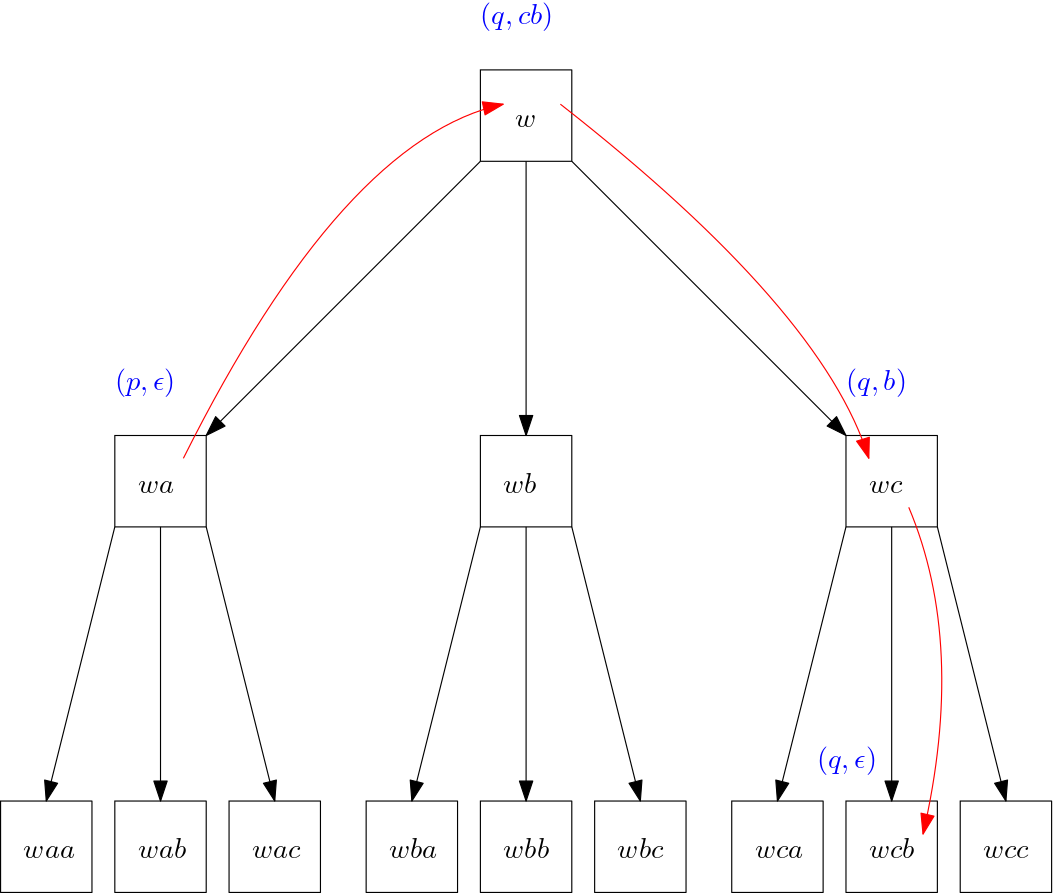
\includegraphics[width=0.66\textwidth]{figures/stack_simulation}
	\caption{Transition $(p, a, \emptyset, q, cb)$ of the RPDS
	%(long arrow)
	 simulated by the PATWA.}
	 \label{stack simulation}
	\end{figure}
\end{center}


Moving up or down the tree structure is enough in order to simulate the modifications of the stack
performed by transitions of $\mathcal{Z}$. Additionally, dropping or lifting pebble is enough to simulate the dropping or lifting of pebbles in the PPDS. As an example, we simulate
$(q, a, 0, \emptyset, q', \text{\textit{drop}})  \in   \Delta_{\mathcal{Z}} $ by the single move $\text{\textit{drop}}$, and
$(q, a, i, \{i\}, q', \text{\textit{lift}})  \in   \Delta_{\mathcal{Z}} $ by the single move 
$\text{\textit{lift}}$. Additionally, we simulate checks against pebble sets in $\mathcal{Z}$ by similar checks in the PATWA.


More formally now, the control states of $\mathcal{A}$ are tuples
from $( Q \times ext_2(\Gamma) )^*$  
composed of a control state of  $\mathcal{Z}$, and
a sequence of elements of $ ext_2(\Gamma)$.

The sequence of letters is used to remember the letters the automaton has to write. 
Each sequence of letters has at worst the length of a corresponding output of the transition relation of $\mathcal{Z}$, hence the sequences of letters of $\Gamma$ are more precisely elements of $\Gamma^{ \leq |\Delta_{\mathcal{Z}}|}$.  


From a state $(q, \epsilon)$, for a transition
$(q, a, i, S, q', x) \in \Delta_{\mathcal{Z}}$,
the automaton's first move simulating the transition, be it the dropping of a pebble, the lifting of a pebble, or going up the tree, is accompanied by 
checks that the pebbles $1, \ldots, i$ are placed on the tree \---- or that no pebble is on the tree if $i=0$ \---- and checks against the presence of the pebbles of $S$.

From a state $(q , bx)$ ($bx \neq \epsilon$ because $b  \in  \Gamma$) the automaton goes down
in direction $b$, that is to say writes $b$, whatever it reads, and remembers the
(sub)word $x$ it still has to write and the state $q$ of the pushdown system. 


If $q  \in  Q_1$ then $ (q,w)  \in  V_1$ for all $w \in \Gamma^{ \leq |\Delta_{\mathcal{Z}}|}$
and
$\mathcal{A}$
executes from $(q,\epsilon)$ all the possible moves of player $1$, to ensure that player $0$ can win after
each of these moves. But if $q  \in  Q_0$, $\mathcal{A}$ in $(q,\epsilon)$ chooses nondeterministically a move of
player $0$ and tries to make player $0$ win. \newline


The priority mapping of $\mathcal{A}$ is almost the same as the one of 
$\mathcal{G}_{\mathcal{Z},Q_0,Q_1,\Omega}$: 
$\Omega_\A(q, x) =
\Omega (q)$. 
The initial state of $\mathcal{A}$ causes it to go deterministically to the starting
configuration of the game.




\begin{lemma}~\label{lemma reduction PATWA}
Player $0$ has a winning strategy from $(q_I, \$, f_I)$ in $\mathcal{G}_{\mathcal{Z},Q_0,Q_1,\Omega}$ iff $\mathcal{A}$ accepts the full
infinite tree $\Gamma^* $.

\end{lemma}


This concludes our construction for the proof of Theorem~\ref{theorem reduction PATWA}.















\end{document}

















